\documentclass[12pt]{article}
\usepackage[T1]{fontenc}
\usepackage[utf8]{inputenc}
\usepackage[margin=1in]{geometry}
\usepackage{graphicx}
% \usepackage{caption} % optional; comment out if not installed
% \usepackage{titlesec}

% --- Code listing (pretty Python) ---
% \usepackage{listings}
% % \usepackage{xcolor}
% \lstdefinestyle{mypython}{
%   language=Python,
%   basicstyle=\ttfamily\small,
%   numbers=left,
%   numberstyle=\tiny\color{gray},
%   stepnumber=1,
%   numbersep=8pt,
%   frame=single,
%   rulecolor=\color{black!20},
%   showstringspaces=false,
%   tabsize=2,
%   breaklines=true,
%   keywordstyle=\color{blue!60!black},
%   commentstyle=\color{gray!70},
%   stringstyle=\color{green!40!black}
% }
% If listings/xcolor aren't available, comment the 3 lines above and wrap code in \verbatim instead.

\title{Visualization Design: Antibiotics and Bacterial Sensitivity}
\author{Chris Low}
\date{\today}

\begin{document}
\maketitle
\renewcommand{\baselinestretch}{1.2}\normalsize

\section*{Visualization and Rationale}

The main idea I want to communicate is how the three antibiotics—Penicillin, Streptomycin, and Neomycin—perform differently depending on whether the bacteria are Gram-positive or Gram-negative. This contrast is clearest in Penicillin, which is highly effective against Gram-positive bacteria but far less effective for Gram-negative ones. Streptomycin and Neomycin don’t show the same sharp divide. Instead, their MIC values are more evenly distributed across both groups, with some Gram-positive species showing resistance and some Gram-negative species showing sensitivity. This contrast between drug profiles is the story I want people to pick up quickly when they look at the figure.

I chose boxplots as the main mark because they give a compact view of the median and spread of MIC values for each antibiotic, letting viewers compare overall effectiveness at a glance. To make sure individual species aren’t lost in the summary, I layered in jittered points with low opacity. This keeps the overall structure clean while still showing where individual bacteria fall. I used a log scale on the y-axis because the MIC values range from about $10^{-3}$ to $10^{3}$, and a linear scale would have squashed all the lower values together. The log scale spreads these values out evenly, making both small and large differences visible. The antibiotics are sorted by median MIC so the ranking is immediately clear, and color is used only to highlight Gram stain, keeping the design focused and uncluttered.


The transformations behind the figure were minimal but purposeful: cleaning and normalizing the column names, reshaping the dataset into a long format for tidy plotting, coercing values to numeric, and filtering out nonpositive values so the log scale is valid. This keeps the visualization grounded in the original data without unnecessary processing. The x-offset between Gram groups helps separate overlapping summaries, and jittering avoids stacked points, so both the structure and the variation are easy to see.

This design naturally emphasizes group-level trends and trade-offs. Because the focus is on Gram stain groups and antibiotic effectiveness, it’s not easy to follow how a single species behaves across all three antibiotics—that would require something like a slopegraph or heatmap. Species names aren’t shown directly on the plot to avoid overcrowding, and the boxplots can make the data look smoother than it really is given the small sample size. Even so, the choice of boxplots, jittered points, log scaling, and sorted categories is deliberate: these elements work together to make the main story—the relationship between Gram stain and antibiotic effectiveness—immediately visible in a single, static image.

\begin{figure}[h!]
  \centering
  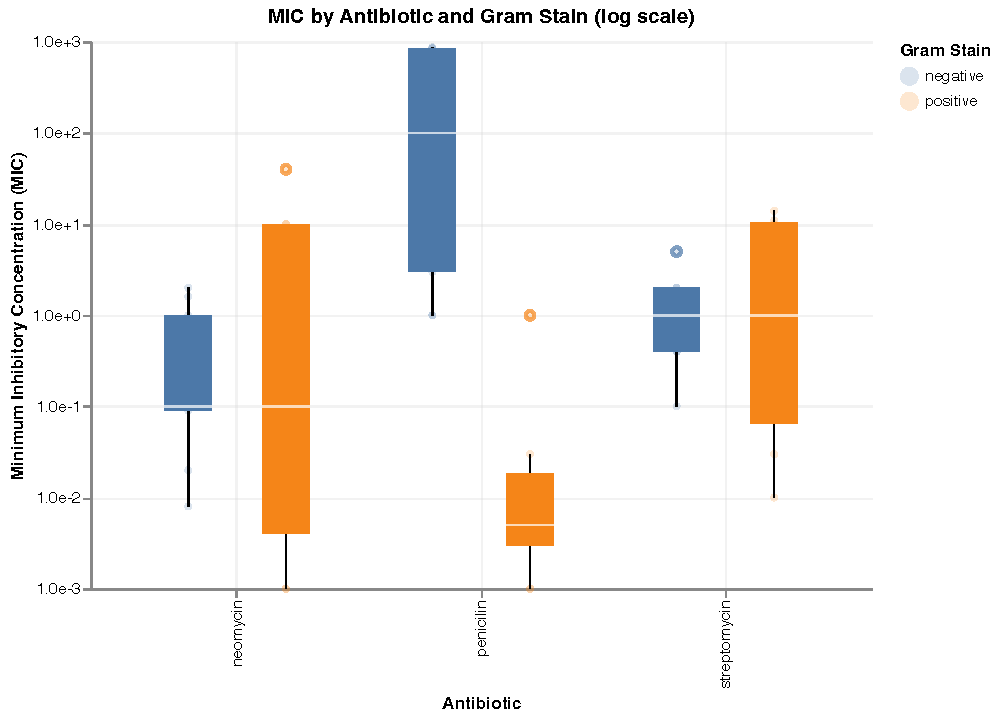
\includegraphics[width=0.9\textwidth]{antibiotics_single_chart.pdf}
  \caption{Distribution of MIC values (log scale) for three antibiotics by Gram stain. Boxplots show overall distribution; points show individual species.}
\end{figure}

\subsection*{Tools and Workflow}
I cleaned and reshaped the CSV in \textbf{Python} using \texttt{pandas} (column normalization; melt to long format; numeric coercion; filtering MIC\,$>$\,0). I built the chart in \textbf{Altair} (Vega-Lite) with boxplots plus jittered points, log scaling on MIC, and antibiotic sorting by median MIC. I exported an SVG and converted it to PDF via \texttt{rsvg-convert}. The write-up and figure were assembled in \textbf{LaTeX} using VS Code with the LaTeX Workshop extension.

\clearpage
\section*{Appendix: Generation Code (Python)}
\begin{verbatim}
import pandas as pd
import altair as alt
import os

df = pd.read_csv("data/antibiotics-1.csv")
df.columns = (df.columns
              .str.strip()
              .str.replace(r'[\s\-]+', '_', regex=True)
              .str.replace('[^0-9a-zA-Z_]', '', regex=True)
              .str.lower())

long = df.melt(
    id_vars=["bacteria", "gram_staining"],
    value_vars=["penicilin", "streptomycin", "neomycin"],
    var_name="antibiotic",
    value_name="mic"
).dropna(subset=["mic"])

long["mic"] = pd.to_numeric(long["mic"], errors="coerce")
long = long[long["mic"] > 0]

antibiotic_order = (long.groupby("antibiotic")["mic"]
                    .median()
                    .sort_values()
                    .index
                    .tolist())

y_axis = alt.Y(
    "mic:Q",
    title="Minimum Inhibitory Concentration (MIC)",
    scale=alt.Scale(type="log", domain=[1e-3, 1e3]),
    axis=alt.Axis(values=[1e-3, 1e-2, 1e-1, 1, 10, 100, 1000], format=".1e")
)

points = (
    alt.Chart(long)
    .transform_calculate(jitter="(random()-0.5)*8")
    .mark_circle(size=20, opacity=0.2)
    .encode(
        x=alt.X("antibiotic:N", sort=antibiotic_order, title="Antibiotic"),
        xOffset=alt.X("gram_staining:N", title=None),
        y=y_axis,
        color=alt.Color("gram_staining:N", title="Gram Stain"),
        tooltip=["bacteria", "antibiotic", "mic", "gram_staining"]
    )
)

boxes = (
    alt.Chart(long)
    .mark_boxplot(size=30)
    .encode(
        x=alt.X("antibiotic:N", sort=antibiotic_order, title="Antibiotic"),
        xOffset=alt.X("gram_staining:N", title=None),
        y=y_axis,
        color=alt.Color("gram_staining:N", title="Gram Stain")
    )
)

final_chart = (points + boxes).properties(
    width=500, height=350,
    title="MIC by Antibiotic and Gram Stain (log scale)"
).configure_axis(grid=True, gridColor='lightgray', gridOpacity=0.3
).configure_view(strokeWidth=0)

final_chart.save("antibiotics_single_chart.svg")
os.system("rsvg-convert -f pdf -o antibiotics_single_chart.pdf antibiotics_single_chart.svg")
\end{verbatim}

\end{document}
